\appendix

\section{Models}
\label{app:models}

Table~\ref{tab:models} lists the 24 models.
All weights are public Hugging Face checkpoints: GPT-2 \citep{radford2019language}, Pythia \citep{biderman2023pythia}, Llama~2 and Llama~3 \citep{touvron2023llama,grattafiori2024llama}, Mistral \citep{jiang2023mistral}, Gemma~2 and Gemma~3 \citep{gemma2024gemma2,gemma2025gemma3}, Qwen2.5 \citep{qwen2024qwen25} and Qwen3 \citep{yang2025qwen3}.
Pythia-410M is the seed-1 checkpoint of the Pythia suite.
Log-probabilities are computed on the jointly tokenized prime and target, with the prime preceded by the beginning-of-sequence token and separated from the target by a space.
A target token counts toward the continuation if its character span starts at or after the continuation's first character.
Priming scores were computed in bfloat16.
Patching runs used float32 for models up to 8B parameters, where the cached and the full-sequence computations agree to $10^{-4}$ nats, and bfloat16 for Qwen2.5-32B and Llama-3.1-70B, which ran on two GPUs.
Sampled completions were generated with vLLM \citep{kwon2023vllm} using temperature 1, top-$p$ 1, at most 24 new tokens and a stop at the first line break.

\begin{table*}[t]
\centering\footnotesize
\setlength{\tabcolsep}{3pt}
\begin{adjustbox}{max width=\textwidth}
\begin{tabular}{lllcccccccc}
\toprule
Model & Size & Type & Disc. & Held-out & \cond{nom} & \cond{pass} & Christianson & Sampled & Patching & Context\\
\midrule
\rows{tables/models.tex}
\bottomrule
\end{tabular}
\end{adjustbox}
\caption{The 24 models and the experiments they enter. Disc.: discovery set (\S\ref{sec:residue}, \S\ref{sec:twoforces}). Held-out: 48 held-out families. \cond{nom}: case disambiguation. \cond{pass}: passive primes. Christianson: items of \citet{christianson2001}, used for the prospective test of \S\ref{sec:twoforces} and for comprehension questions (\S\ref{sec:transfer}). Sampled: sampled completions. Patching: \S\ref{sec:mechanism}. Context: Appendix~\ref{app:e014}.}
\label{tab:models}
\end{table*}

\section{Materials}
\label{app:materials}

The discovery families come from the released items of \citet{amouyal2025} and from the NP/Z subset of the SAP benchmark \citep{huang2024}.
For each family we wrote the comma version (\cond{cue}), the transitive versions with a resumptive pronoun (\cond{tb}, \cond{tc}), and the two intransitive versions (\cond{nb}, \cond{nc}).
The intransitive verbs (\ex{slept, yawned, sneezed, laughed, sighed, snored, napped, shivered, dozed, frowned, giggled, rested}) cannot take an object, and each family uses one of them with the family's own subject.
The held-out families combine 24 items with reflexive-absolute verbs from \citet{cehakova2025} with 24 NP/Z items from SyntaxGym \citep{gauthier2020}.
The two sources differ in the object expectation of their verbs (about $-0.3$ and $1.5$ nats on average), which is why we report between-family slopes on the held-out set with source fixed effects.
The items of \citet{christianson2001} were transcribed from the published appendix.
They comprise 42 optionally transitive and 12 reflexive-absolute verbs, each with a short and a long ambiguous region (\ex{the deer} against \ex{the deer that was brown and graceful}) and, for the optionally transitive verbs, a plausible and an implausible object.
Primes from this set are followed by a fixed set of 48 discovery families as targets, excluding any target that shares a content word with the prime.

A target never shares a content word with its prime, which removes lexical repetition as a source of priming.
In the discovery set each prime is paired with 78 to 92 targets.
The $L$ measure compares two strings that contain the same words in the same order and differ only in the position of the comma.
The $S$ measure scores only the first word of the main clause, so its value does not depend on the length of the continuation.

\section{Statistics}
\label{app:stats}

For a model and a contrast, we first average the measure over targets for every prime family and condition, then average over prime families.
Intervals resample prime families and target families independently with replacement (1,000 draws) and recompute the contrast, which treats both as random samples of items.
Item-level regressions (Figure~\ref{fig:slopes}) regress the family-level contrast on the two standardized predictors with heteroskedasticity-consistent standard errors.
Across models we pool per-model estimates with the random-effects estimator of \citet{dersimonian1986}, taking the standard error of each model's estimate from its bootstrap interval.
Models are not a random sample of language models, so we read the pooled value as the typical model of our panel and always report how many models show the effect.
Table~\ref{tab:residue} gives the residue of every model on the three item sets, and Figure~\ref{fig:slopes} the item-level regressions of \S\ref{sec:twoforces}.

\begin{figure*}[t]
\centering
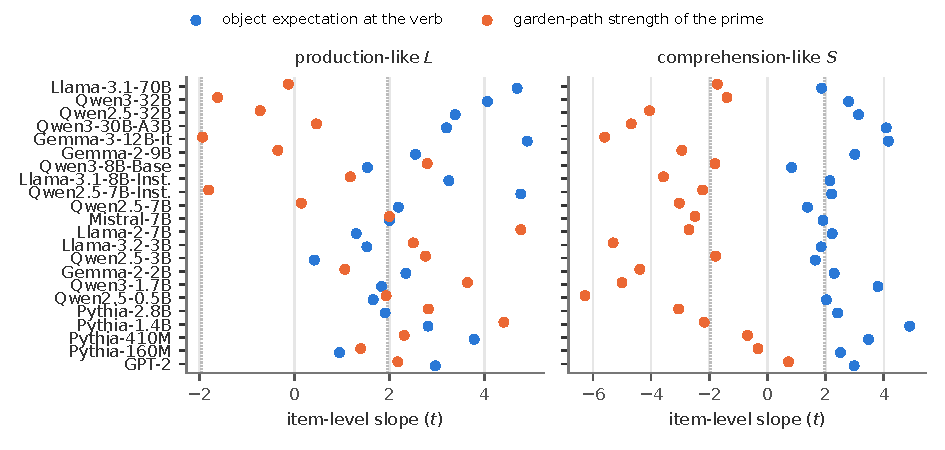
\includegraphics[width=\textwidth]{figures/fig_slopes}
\caption{Item-level predictors of the residue on the discovery set. Each point is the $t$ value of one predictor in a regression of the family-level contrast $A$ on the model's object expectation after the ambiguous verb (blue) and on the garden-path strength of the prime, the surprisal of its disambiguating word without versus with the comma (orange). Dotted lines mark $|t|=1.96$. Object expectation raises $A$ on both measures. Garden-path strength lowers it on the comprehension-like measure $S$ in 21 of 22 models.}
\label{fig:slopes}
\end{figure*}


\begin{table}[t]
\centering\footnotesize
\setlength{\tabcolsep}{2pt}
\begin{adjustbox}{max width=\columnwidth}
\begin{tabular}{lccc}
\toprule
Model & Discovery & Held-out & Christianson\\
\midrule
\rows{tables/residue_sets.tex}
\bottomrule
\end{tabular}
\end{adjustbox}
\caption{Residue $A_L$ (nats) with 95\% two-way bootstrap intervals on the three item sets. Dashes mark models not run on a set.}
\label{tab:residue}
\end{table}

\section{Pre-specified Predictions and Outcomes}
\label{app:prereg}

Each confirmatory experiment was preceded by a dated record of its design, predictions and analysis, committed to version control before any of its data were collected.
Table~\ref{tab:prereg} lists every prediction and its outcome.
Three experiments did not confirm what we expected.
On the held-out families, the between-family relation between object expectation and the residue was measured on $S$ and was confirmed in only 6 of 15 models, whereas the error relation was confirmed in 9 of 15.
Figure~\ref{fig:slopes} shows that object expectation predicts the residue on both measures within the discovery set, and the held-out result indicates that the relation is weaker on $S$ when the families come from sources that differ in verb class.
For NP/S garden paths neither force appeared, which led to the scope statement of \S\ref{sec:twoforces}.
The context manipulation of Appendix~\ref{app:e014} failed its manipulation check.

The within-family manipulation of the error used continuations generated to follow each fixed prefix and checked for grammaticality.
Each family had between four and eight continuations whose disambiguating words differed in surprisal.
The effect of the error remained when only human-written continuations were used, when a naturalness score of the continuation was added as a covariate, and when continuations beginning with an auxiliary were removed ($t$ between $-2.8$ and $-6.2$ in the three models with an error effect).

\begin{table*}[t]
\centering\small
\setlength{\tabcolsep}{4pt}
\begin{tabular}{p{2.6cm}p{6.6cm}p{5.6cm}}
\toprule
Experiment & Pre-specified prediction & Outcome\\
\midrule
Held-out families & (i) object expectation predicts the residue on $S$ (ii) error predicts it with the sign found in discovery (iii) sign of the net residue & (i) 7/17 \emph{(not confirmed)} (ii) 11/17, same sign in 16/17 (sign test $p=.0001$) (iii) 5/9\\
Within-family error & more surprising disambiguation lowers the residue in the models with a discovery error effect & confirmed in 3/3, and null in the 2 models predicted null\\
NP/S & the two forces generalize to NP/S garden paths & \emph{not confirmed} (1/5 and 0/4)\\
MV/RR & error and commitment relations in main-verb/reduced-relative garden paths & (i) error 6/9 (ii) commitment 0/8\\
Case (\cond{nom}) & (i) object expectation predicts the residue without punctuation (ii) error relation negative (iii) comma part of the predictor vanishes & (i) 22/22 (ii) 20/22 (iii) \emph{not confirmed} (reinterpreted as part of object expectation)\\
Measures & (i) residue on $L$ positive (ii) error relation stronger on $S$ than on $L$ & (i) 16/16 (ii) 14/16\\
Passive (\cond{pass}) & passive residue small relative to \cond{gp} & median ratio 0.12 (confirmed)\\
Sampled text & (i) residue positive (ii) raw \cond{gp}$-$\cond{cue} contrast positive (iii) style alignment (iv) size follows $A_L$ & (i) 11/12 (ii) \emph{4/12} (iii) 12/12 (iv) $\rho=0.81$\\
Patching & (i) NP retains $\le 50\%$ and less than MC on $L$ (ii) MC changes $S$ more than NP & (i) 7/9 (ii) 8/9\\
Context & manipulation check on object expectation at the verb & \emph{not met} (0/11)\\
\bottomrule
\end{tabular}
\caption{Pre-specified predictions and outcomes. Counts are models in which the prediction held. Outcomes that did not confirm the prediction are in italics.}
\label{tab:prereg}
\end{table*}

\section{Patching}
\label{app:patching}

For a prime with noun-phrase tokens $N$ and main-clause tokens $M$, we run the prime twice.
The original run keeps all states.
The counterfactual run overwrites, at the output of every layer, the residual-stream vectors at $N$ with the vectors of the same tokens from the donor prime, and recomputes all positions after $N$ with these vectors in place.
Since the models use rotary position embeddings, the residual stream carries no absolute position, and the one-token offset introduced by the donor's comma does not need correction.
The target is then scored against a key--value cache that takes the counterfactual run's keys and values at the positions of the chosen span and the original run's elsewhere.
The prediction of the target's first token comes from the run that supplies the prime's last token.
Table~\ref{tab:patching} gives all estimates with intervals.
In the depth analysis the overwrite starts at layer $\lfloor fL \rfloor$ for $f \in \{0.25, 0.5, 0.75\}$, so that the noun phrase's keys and values below that layer keep the object analysis.
The retained fractions when the overwrite starts at a quarter, half and three quarters of the depth are 0.51 (0.41, 0.61), 1.07 (1.01, 1.12) and 1.01 (1.00, 1.01) for Llama-3.1-8B-Instruct, 0.56 (0.45, 0.65), 1.06 (1.02, 1.12) and 1.02 (1.01, 1.04) for Mistral-7B, and 0.22 (0.02, 0.35), 0.44 (0.28, 0.55) and 1.04 (1.01, 1.08) for Qwen2.5-7B.
Replacing both the noun phrase and the main clause retains 0.32 to 0.67 of the residue, more than replacing the noun phrase alone, because it also removes the adaptation.
For the role direction we take, at each layer, the difference between the mean noun-phrase states of object primes without a comma (\cond{tb}) and subject primes without a comma (\cond{nb}), fit without the prime's own family.
In the middle half of the layers the projection of the noun-phrase states on this direction is set to the subject mean, and the same shift along three norm-matched random directions serves as control.
The residue retained is 0.50 to 0.92 with the role direction and 0.42 to 0.83 with random directions, and the role direction retains less in Llama-3.2-3B, Llama-3.1-8B-Instruct and Qwen2.5-32B.
A direction fit on object primes against subject primes with a comma retains 0.31 to 0.74, less than random directions in all seven models, but it also separates primes with and without a comma.

\begin{table*}[t]
\centering\small
\setlength{\tabcolsep}{4pt}
\begin{tabular}{lccccc}
\toprule
Model & $A_L$ & $\rho$, NP & $\rho$, MC & $\Delta A_S$, NP & $\Delta A_S$, MC\\
\midrule
\rows{tables/e013_ci.tex}
\bottomrule
\end{tabular}
\caption{Patching results with 95\% two-way bootstrap intervals. $\rho$: retained fraction of the residue on $L$. $\Delta A_S$: change of the residue on $S$ in nats. NP and MC: the target reads counterfactual states at the noun phrase or at the main clause.}
\label{tab:patching}
\end{table*}

\section{Context Manipulation}
\label{app:e014}

Each of 87 discovery families received five context sentences, written by Qwen3-32B from a fixed instruction and checked automatically for length, the absence of commas, and the absence of the family's verbs and main-clause words.
Two contexts present the noun phrase as the subject's goal (\ex{The man had been tracking the deer since dawn.}), two present the subject and the noun phrase as doing unrelated things (\ex{The man studied the map while the deer drifted downstream.}), and one only places them together.
Six families for which no context passed the checks were dropped as specified.
Each context precedes all four primes of Equation~\ref{eq:A}, so the context's direct effect on the target cancels.

The specified manipulation check required object expectation after the ambiguous verb to be higher after goal contexts in more than 70\% of families.
It rose on average in every model but in only 48\% to 64\% of families, so the confirmatory test is uninformative by its own criterion.
The contexts did change the garden path itself: the surprisal of the disambiguating word without versus with the comma rose by 0.9 to 1.7 nats (Table~\ref{tab:e014}).
This analysis was added after the first two models had been scored.
Under it, the residue on $S$ is larger after goal contexts in 10 of 11 models, which runs against an account in which the prime acts only through its disambiguation error, since that error also grows.

\begin{table}[t]
\centering\footnotesize
\setlength{\tabcolsep}{2.5pt}
\begin{adjustbox}{max width=\columnwidth}
\begin{tabular}{lccccc}
\toprule
Model & $\Delta$exp. & fam. & $\Delta$GP & $\Delta A_L$ & $\Delta A_S$\\
\midrule
\rows{tables/e014.tex}
\bottomrule
\end{tabular}
\end{adjustbox}
\caption{Context manipulation, goal minus unrelated contexts. $\Delta$exp.: object expectation at the verb (pre-specified check), and the share of families in which it rose. $\Delta$GP: garden-path strength. $\Delta A_L$, $\Delta A_S$: change of the residue, with standard errors over families.}
\label{tab:e014}
\end{table}

\section{Overridden Statements}
\label{app:facts}

The 200 items combine ten frames (meeting day, location of objects, city of residence, start time, favourite colour, due month, profession, material, instrument, language) with five entities and two pairs of values in both orders.
Every context starts with a short label (\ex{Note:}, \ex{Mistake:}), so that the overridden statement is tokenized identically in all conditions.
The measure is $M=\log P(A)-\log P(B)$ after the probe, and $R=M_{\text{CORR}}-M_{\text{CTRL}}$.
In the re-encoding test, the residual-stream states of the overridden statement's tokens in CORR are replaced at every layer by those of the same tokens in PRE, where \ex{Mistake:} precedes the statement, and the same replacement in CTRL is subtracted.
This leaves the pull largely intact (Table~\ref{tab:facts}), as the pre-specified prediction did not expect.
The knockout analysis uses full sequences with a four-dimensional attention mask that blocks the listed query--key pairs in every layer and head.
Retained fractions of the pull, for blocking the answer's access to the statement, the answer's access to the value token only, and all later positions' access to the statement, are 1.10, 0.94, 0.12 (Llama-3.2-3B); 1.64, 1.53, 0.21 (Llama-3.1-8B-Instruct); 1.34, 1.10, $-$0.06 (Mistral-7B); 2.08, 1.70, $-$0.03 (Qwen3-8B-Base); 1.12, 1.11, 0.16 (Gemma-2-9B); 0.16, $-$0.04, 1.13 (Qwen2.5-7B); 0.48, 0.66, $-$0.20 (Llama-3.1-70B); and $-$3.02, $-$3.39, 2.90 (Qwen2.5-32B, whose small pull of 0.56 nats reverses).

\begin{table}[t]
\centering\footnotesize
\setlength{\tabcolsep}{3pt}
\begin{adjustbox}{max width=\columnwidth}
\begin{tabular}{lcccc}
\toprule
Model & $R$ & CORR$-$PRE & $\rho$ CLAIM & $\rho$ FULL\\
\midrule
\rows{tables/e015.tex}
\bottomrule
\end{tabular}
\end{adjustbox}
\caption{Overridden statements (nats). $R$: pull of the overridden value beyond a matched mention. $\rho$: retained fraction of $R$ after re-encoding the overridden statement (CLAIM) or the whole context (FULL).}
\label{tab:facts}
\end{table}

\section{Coding of Sampled Completions}
\label{app:coding}

Sampled continuations of \ex{While}~$s$~$v$ are coded from part-of-speech tags, because a dependency parser is itself misled by comma-less input of exactly this kind.
A continuation that begins with punctuation is intransitive.
One that begins with an object pronoun, or with a noun phrase that is followed by punctuation, a second noun phrase or the end of the clause, is transitive.
A noun phrase followed by a finite verb is intransitive, and if no comma precedes it, the continuation is itself a garden-path sentence.
A second version of the rules also resolves coordination after the noun phrase.
Continuations with a relative clause or an unresolved coordination after the noun phrase are coded as ambiguous and excluded (1.5\% to 13\% per model).
On 1,066 sentences from our materials with known structure the rules are correct on 1,063.
On 180 generated continuations sampled across classes, one annotator judged 27 to 29 of 30 transitive codes and 29 of 30 intransitive codes correct.
The results of \S\ref{sec:residue} and \S\ref{sec:transfer} use the first version, and the second gives the same conclusions with the residue positive in 12 of 12 models.
